% !TeX root = ../main.tex
% Add the above to each chapter to make compiling the PDF easier in some editors.

\chapter{Evaluation}\label{chapter:evaluation}

We evaluate our model's performance and compare it to other work.
This answers the three research questions posed in Chapter~\ref{chapter:introduction}: how accurately a decision tree model predicts PostgreSQL query runtimes, which of T3's key concepts transfer effectively, and how competitive the result is against existing learned cost models.
Unless otherwise noted due to the nature of the evaluation, all results are evaluated on actual cardinalities.
Therefore, we detach our results from the ongoing issue of accurately estimating cardinalities~\parencite{leis2018job}.

\paragraph{Environment.}
Model training and evaluation for the results reported in this thesis were run on a personal laptop: an Apple MacBook Pro (16-inch, 2021) with the Apple M1 Pro processor (10 CPU cores, 16 GPU cores), 16\,GB memory, and a 512\,GB SSD, under macOS 15.7.3.

\section{Generalization and Frequency Distribution}

\paragraph{Accuracy and Generalization across Databases.}
Figure~\ref{fig:database_q} shows the generalization capabilities of our model across different, unseen database instances.
This is ensured by training the model on all databases except the one being tested.

The median Q-Error (p50) stays below 1.33 for all databases,
ranging from 1.07 (Walmart) to 1.32 (Basketball),
indicating consistently good accuracy on unseen databases.
We observe that the p90 and average values show more variation across databases:
p90 ranges from 1.30 (Walmart) to 3.32 (Basketball),
and the average from 1.13 (Walmart) to 2.92 (Hepatitis).
This reflects that a small number of harder-to-predict queries
drive up the tail and mean errors for some databases.
Despite the increased variation in the average and p90 values, we conclude that the model can generalize across unseen database instances within the ZeroShot workload.
We scope this finding to the ZeroShot query pattern~\parencite{zeroshot}.
Generalization to more structurally diverse queries remains untested and is addressed in the future work (Chapter~\ref{chapter:future_work}).

Since we trained on the same data as the ZeroShot model, it is reasonable to compare the median values of our model to theirs.
As their median values across databases are in the same range~\parencite{zeroshot}, we infer that our model has a comparable generalization performance.

\paragraph{Frequency Distribution.}
Figure~\ref{fig:qerror_freq} shows the Q-Error frequency distribution of our model on the JOB benchmark
(which we use further in the evaluation).
The distribution is heavily right-skewed: the majority of the 77 queries are predicted with a Q-Error
close to 1, with a median of 1.33.
However, a small number of queries have considerably higher errors,
pulling the average up to 1.89 and the 90th percentile to 3.41,
with the worst-predicted query reaching a Q-Error of 7.43.
This skewed distribution explains the general pattern visible in Figure~\ref{fig:database_q}:
the p50 stays low and stable across databases,
while the average and p90 are more sensitive to a few hard-to-predict outliers.
\begin{figure}[htpb]
  \centering
  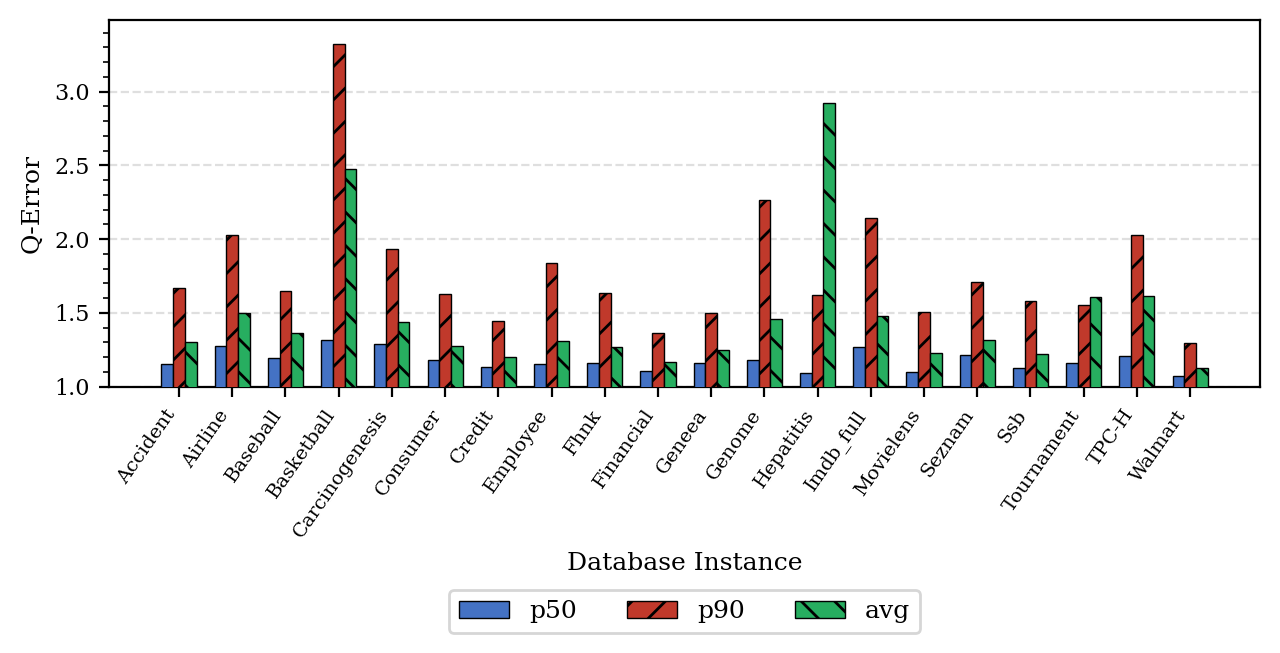
\includegraphics[width=\textwidth]{figures/database_q.png}
  \caption[Q-Error across Database Instances]{Q-Error (p50, p90, and average) of our model evaluated across all database instances. Each database is excluded from the training set when tested and plotted. All other databases are included in the training set. }\label{fig:database_q}
\end{figure}

\begin{figure}[htpb]
  \centering
  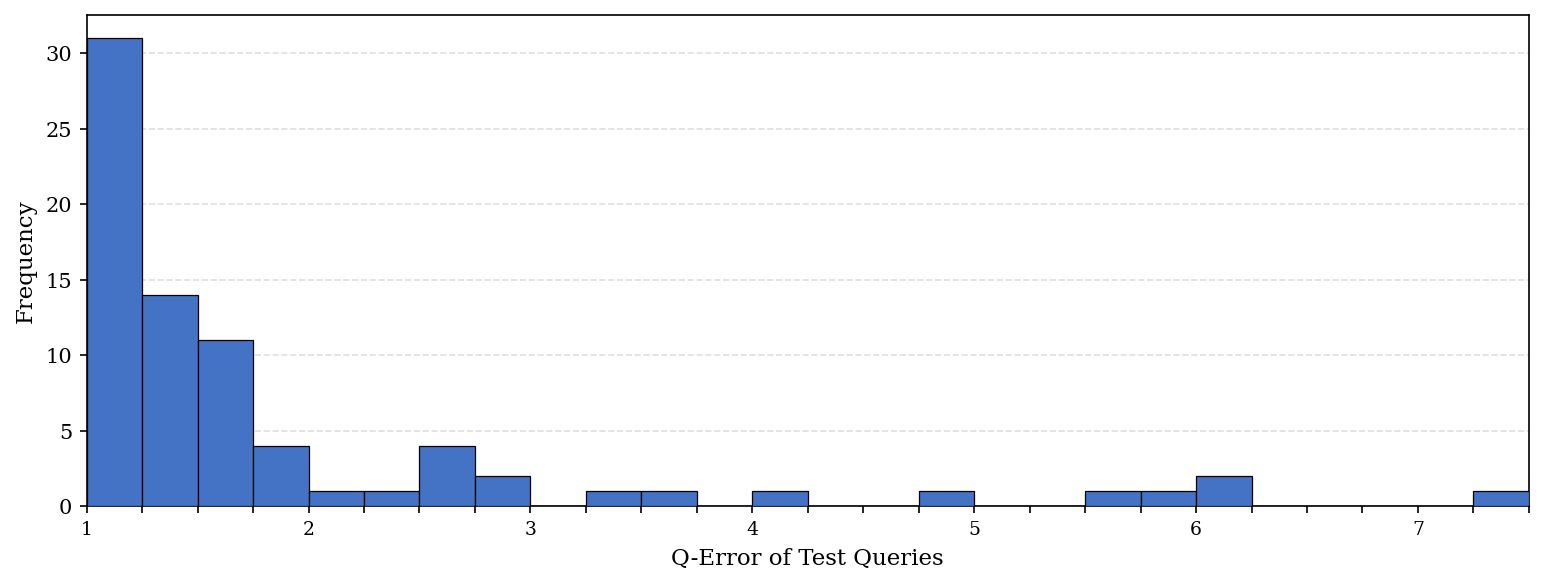
\includegraphics[width=\textwidth]{figures/qerror_freq.png}
  \caption[Q-Error Frequency Distribution]{Frequency distribution of Q-Error values across all available JOB queries.
  The model is trained on all databases except IMDB, which is the database of the JOB-Benchmark.}\label{fig:qerror_freq}
\end{figure}

\section{Comparison to Other Models}

\paragraph{Comparison to T3 (Umbra) and ZeroShot.}

The original T3 model for Umbra by Rieger and Neumann~\parencite{t3} and the ZeroShot model~\parencite{zeroshot} offer very good generalization performance across unseen databases.
Because T3 (Umbra) uses different queries for generalization testing, we cannot directly compare the generalization performance of our model to theirs.
But, Rieger \& Neumann compared both models on the JOB-Benchmark and reported excellent performance for both models~\parencite{t3}.

We also have JOB queries available for evaluation, so we can compare the models on that.
In the original comparison, Rieger \& Neumann compare the p50, p90, and average Q-Error values.
They had all 113 JOB queries available for evaluation. 

However, the provided ZeroShot training data came with data limitations.
Namely, longer-running queries are not included~\parencite{zeroshot}, so we only have 77 JOB queries available for evaluation.
As the number of total queries differ, it is not sensible to compare the p50 and p90 Q-Error values directly.
If the missing queries had a very high Q-Error, the p50 value of our model would be higher than now and using the current p50 value would be misleading.
This also applies to the p90 value.

Considering how the median is calculated, we end up with the 57th-best Q-Error value when we take the p75 Q-Error of our model.
The 57th-highest Q-Error (p75) also corresponds to the p50 error of the ZeroShot and T3 (Umbra) models.
Therefore, even if the missing queries had very high errors, the new p50 value would not get worse than the current p75 value.
Hence, we can use it as a lower bound for the median performance of our model and compare it in Figure~\ref{fig:57th_comparison}.

In this case, our model performs worse than the ZeroShot and T3 (Umbra) models on the JOB-Benchmark.
Using the current 57th-best (p75) value for comparison implies a worst-case-scenario for our model.
With lower Q-Errors on the missing queries, the new 57th-highest (p50) value would be lower.

To further narrow down the comparison, we also include the average Q-Error values in Figure~\ref{fig:avg_comparison}.
Although we only have 70\% of the queries available for the calculation on our model, we still see a notable trend. 
Decision trees like T3 offer SOTA performance on average for Umbra, followed by ZeroShot.
Our model, a T3-based implementation for PostgreSQL, tends to perform worse, but the difference on average is smaller than on percentiles.
Thus, it is still a good starting point.

\begin{figure}[htpb]
  \centering
  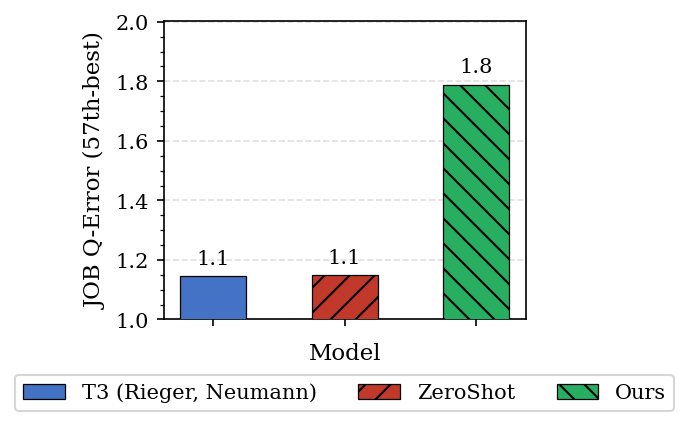
\includegraphics[width=0.7\textwidth]{figures/57th_comparison.png}
  \caption[57th-best Q-Error Comparison between T3 (Umbra), ZeroShot, and Our Model]{57th-best Q-Error on the Join Order Benchmark for T3 (Umbra), ZeroShot, and our model.
  Values for T3 (Umbra) and ZeroShot are taken from Rieger \& Neumann~\parencite{t3}}\label{fig:57th_comparison}
\end{figure}

\begin{figure}[htpb]
  \centering
  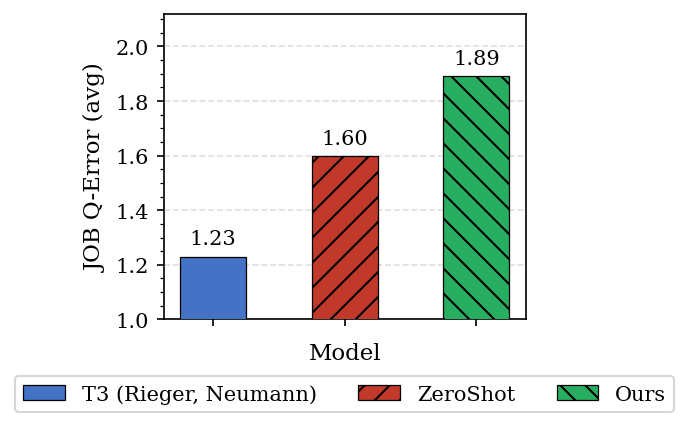
\includegraphics[width=0.7\textwidth]{figures/avg_comparison.png}
  \caption[Average Q-Error Comparison between T3 (Umbra), ZeroShot, and Our Model]{Average Q-Error on the Join Order Benchmark for T3 (Umbra), ZeroShot, and our model.
  Values for T3 (Umbra) and ZeroShot are taken from Rieger \& Neumann~\parencite{t3}.
  Our model's average is calculated over 77 instead of 113 queries.}\label{fig:avg_comparison}
\end{figure}

\paragraph{T3-based Models with Different Feature Vectors.}

Wehrstein et al. ran the JOB-Benchmark on their T3-based model and reported a median Q-Error of 4.07, using estimated cardinalities~\parencite{jobcomplex}.
Like before, they had the full 113 queries at disposal. We again use the 57th-best (p75) Q-Error value for the comparison with our model, this time selecting cardinality estimates to match their setup.

Although we are in the worst-case-scenario, our model clearly outperforms Wehrstein et al.'s model, as Figure~\ref{fig:comp_wehrstein} shows.
A key difference between the models is the used feature vector, where only our model uses a completely PostgreSQL-native feature vector.
Hence, we demonstrate the relevance of PostgreSQL-native features.


\begin{figure}[htpb]
  \centering
  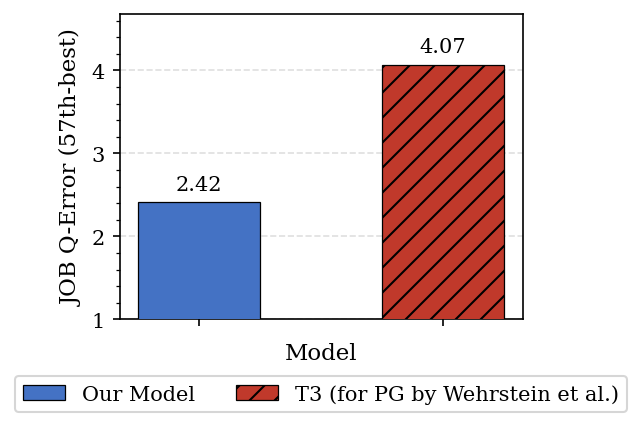
\includegraphics[width=0.7\textwidth]{figures/plot_comp_wehrstein.png}
  \caption[57th-Best Q-Error: Our Implementation vs.\ T3 for PostgreSQL by Wehrstein et al.]{57th-best Q-Error on the Join Order Benchmark. Our model against T3 adapted for PostgreSQL by Wehrstein et al~\parencite{jobcomplex}. Estimated cardinalities. }\label{fig:comp_wehrstein}
\end{figure}



\paragraph{Further PostgreSQL Prediction Models.}

Table~\ref{tab:median_qerror_job} shows the 57th-best Q-Error for different learned cost models on the JOB-Benchmark using PostgreSQL and estimated cardinalities.
As established earlier, we use the 57th-best Q-Error as the comparison metric.
For models evaluated on all 113 JOB queries, the 57th-best value equals the median (p50).
On the other hand, for our model, which has access to only 77 queries, the 57th-best value corresponds to p75 and is therefore a conservative lower bound for our true median.

Here, the best performing models are neural networks like ZeroShot~\parencite{zeroshot} and DACE~\parencite{dace}, with a 57th-best Q-Error below 2.
Our model is in the top 4, coming in at 2.42, even under this worst-case comparison.
The remaining models are neural network-based estimators, such as QPPNet~\parencite{qppnet}.
They show a significant accuracy gap to the top performers, with 57th-best Q-Errors ranging from 8 to 18.
Finally, PostgreSQL's untrained, built-in cost estimator performs worst by a very large margin at a 57th-best Q-Error of over 1000, confirming the need for learned approaches.
Regarding learned approaches, not only neural networks can perform well, but also decision trees like T3 for PostgreSQL.


\begin{table}[htpb]
  \centering
  \begin{tabular}{lc}
    \toprule
    \textbf{Model} & \textbf{57th-best Q-Error} \\
    \midrule
    Postgres (v16)  & 1015.67 \\
    DACE            & 1.91    \\
    E2E             & 13.21   \\
    FlatVector      & 2.15    \\
    MSCN            & 13.85   \\
    NEO             & 13.20   \\
    QPPNet          & 17.50   \\
    QueryFormer     & 8.30    \\
    ZeroShot        & \textbf{1.58}    \\
    Our model       & 2.42    \\
    \bottomrule
  \end{tabular}
  \caption[57th-best Q-Error on JOB across different Models]{57th-best Q-Error on the Join Order Benchmark (JOB) across different models, data from Wehrstein et al.~\parencite{jobcomplex}. For all models except ours, this equals the median (p50), as they are evaluated on the full 113 JOB queries. Our model is evaluated on 77 queries, so its 57th-best value corresponds to p75 -- a conservative lower bound for its true median. Estimated cardinalities.}\label{tab:median_qerror_job}
\end{table}

\section{Ablation Study}\label{sec:evaluation_ablation}
\paragraph{Actual vs. Estimated Cardinalities.}

Figure~\ref{fig:card_comparison} shows prediction accuracy under three cardinality conditions.
For each condition, we used the model variant trained under the matching setting.
Therefore, for a query from database $X$, we used the model
that was trained on all databases except $X$ and used the corresponding cardinality type.
This ensures the correctness of the comparison.

Using exact cardinalities for both training and evaluation gives the best results.
This is a setting of our thesis, where we do not investigate the cardinality estimation issue.
When, for the models trained on actual cardinalities, we switch to estimated cardinalities for evaluation, accuracy degrades.
The median Q-Error increases only moderately,
while the p90 and average Q-Error rise more sharply.
Hence, it reflects that large cardinality estimation errors lead to large performance prediction errors
for a subset of queries, disproportionately affecting the p90 errors and the average~\parencite{t3}.
The same asymmetric degradation pattern has been observed for other performance prediction models~\parencite{stage}.

Training on estimated instead of exact cardinalities partially compensates for this effect.
The model trained and evaluated on estimated cardinalities achieves
a lower average Q-Error than the model trained on exact cardinalities but evaluated on estimated ones.
Thus, this demonstrates that the model can somewhat learn to account for the systematic biases of the cardinality estimator~\parencite{leis2018job}.
However, the p90 Q-Error stays at a similar, high level in both estimated-cardinality settings, indicating that a small number of heavy outliers remain.

We conclude that incorrect cardinality estimates distort performance prediction accuracy substantially.
Cardinality estimation remains an important and unsolved problem~\parencite{leis2018job},
and improvements in cardinality estimation would directly benefit performance prediction.

\begin{figure}[htpb]
  \centering
  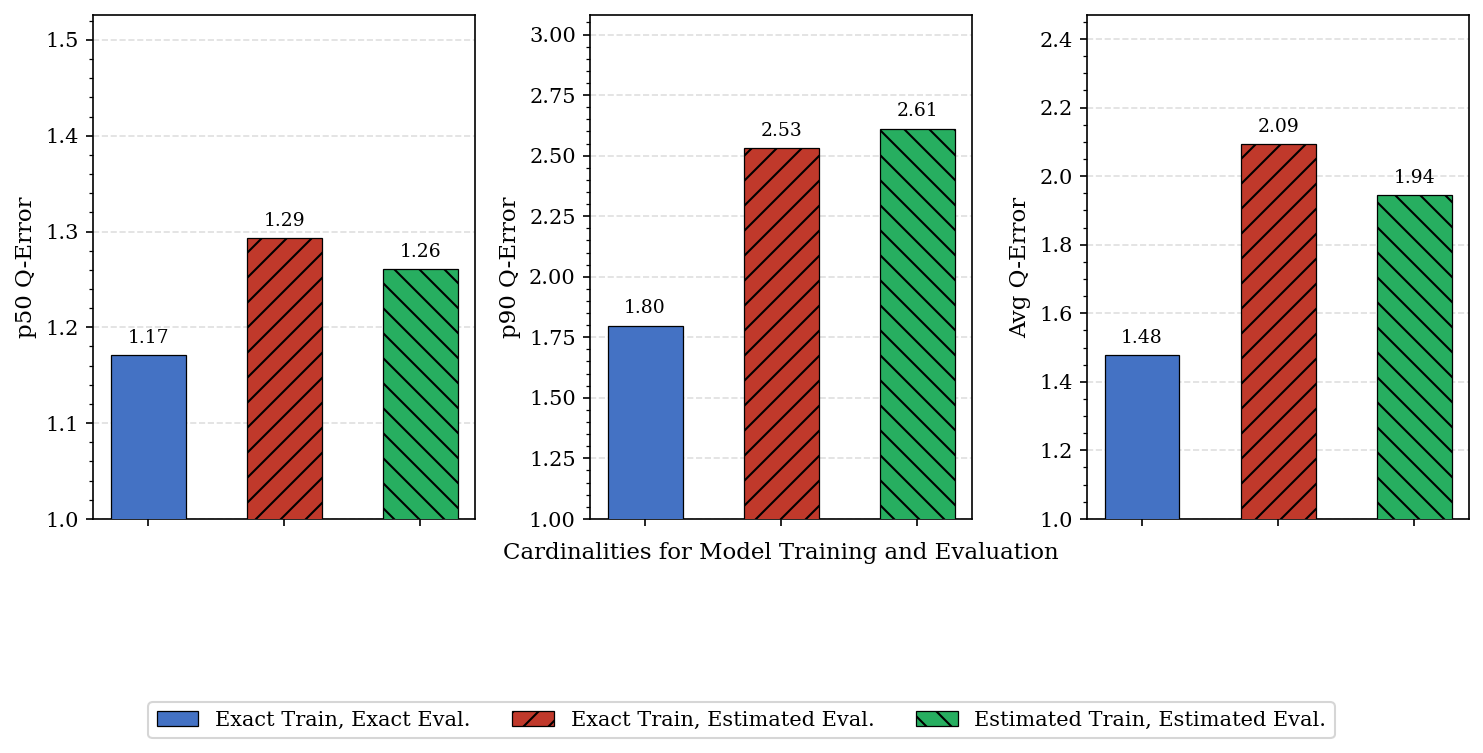
\includegraphics[width=\textwidth]{figures/card_comparison.png}
  \caption[Actual and Estimated Cardinality Comparison]{Q-Error (p50, p90, and average) over all queries under three cardinality settings: trained and evaluated on exact cardinalities, trained on exact but evaluated on estimated cardinalities, and trained and evaluated on estimated cardinalities.}\label{fig:card_comparison}
\end{figure}


\paragraph{Per-Query vs. Per-Pipeline vs. Per-Tuple Targets.}

Figure~\ref{fig:query_pipeline_tuple} compares Q-Error across three prediction granularities:
per-query, per-pipeline, and per-tuple.
This directly copies the evaluation of Rieger and Neumann~\parencite{t3},
who find that finer granularities consistently improve accuracy --
with per-tuple being best and per-query being worst.
We observe the opposite: the per-query model achieves the lowest Q-Error across all three metrics,
while per-pipeline and per-tuple models perform noticeably worse.

The core issue is the reliability of the per-pipeline execution times
that can be extracted from PostgreSQL's output in the ZeroShot dataset~\parencite{postgresql_docs_query_path}.
In Umbra, pipeline breakers require full materialization before any downstream pipeline
can begin scanning their output~\parencite{t3},
making pipelines sequential execution units
whose individual durations sum to the total query time.

Unlike Umbra, PostgreSQL query plans do not expose pipeline execution times directly.
Instead, they must be derived from the per-node durations recorded by
\texttt{EXPLAIN ANALYZE}~\parencite{postgresql_docs_query_path}.

This derivation is fundamentally limited by PostgreSQL's Volcano iterator model~\parencite{graefe1994},
which does not execute pipelines as separate sequential units.
Nodes from different pipelines execute interleaved rather than one after the other.

For example, a hash join operator (belonging to pipeline P1)
builds its hash table by calling \texttt{next()} on its input table scan (belonging to pipeline P0)
one tuple at a time.
The join and the scan therefore execute interleaved over the same wall-clock period:
the join is active from its first \texttt{next()} call to the moment the hash table is complete,
and the scan is active during every individual tuple fetch within that same period.

As a result, \texttt{EXPLAIN ANALYZE} reports two cumulative wall-clock timestamps per node:
the time from query start to when the node produced its first output row,
and the time to when it produced its last row.
These are wall-clock durations, not exclusive execution times --
each node's interval includes the time it spent waiting for its children.
Consequently, both the join (P1) and the scan (P0) receive overlapping time intervals,
even though they belong to different derived pipelines.

To derive pipeline times from these overlapping intervals,
we first compute each pipeline's span as the range from the earliest node start to the latest node stop within that pipeline.
We then assign each pipeline a proportional share of the actual query time,
scaled by its span relative to the total observed plan span.
A correction factor is applied so that the pipeline times sum exactly to the actual query time.

However, this proportional allocation is a heuristic.
Because the node intervals overlap, the raw spans sum to more than the total observed span —
and the correction factor compensates arithmetically rather than recovering the true exclusive execution time of each pipeline.
The individual pipeline labels therefore remain imprecise,
introducing noise into the training targets.

For instance, in plan 2 of \texttt{tpch/workload\_100k\_s1\_c8220},
pipeline P0 (table scan) is recorded from $t = 946$ms to $t = 2{,}156$ms,
giving a span of 1{,}210ms.
Pipeline P1 (table scan, join) is recorded from $t = 0$ms to $t = 2{,}185$ms,
giving a span of 2{,}185ms.
P0 is entirely nested inside P1's time window,
so the raw spans already sum to 3{,}395ms against an actual query time of 2{,}239ms.
The correction factor rescales both pipeline times so their sum is correct on a query level,
but it cannot determine how much of the 2{,}239ms truly belongs to P0 versus P1.

The per-tuple approach, which divides the pipeline runtime into per-tuple runtimes, is additionally weakened by a difference in dataset characteristics.
In T3, the query execution time span is larger than $10^{-5}$\,s to $10$\,s~\parencite{t3}.
Thus, Rieger and Neumann identify this wide range as the primary motivation for the per-tuple approach.
Decision trees have a limited number of discrete leaf values and
struggle to predict accurately over such a large range.
Hence, normalizing by tuple count compresses the prediction target and improves accuracy~\parencite{t3}.
However, in our PostgreSQL dataset, query execution times span a much narrower range,
as visible in Figure~\ref{fig:query_runtime_hist}.

With a narrower range and per-pipeline targets that are already noisy,
the per-tuple decomposition provides no accuracy benefit and introduces additional label inaccuracies instead.

\begin{figure}[htpb]
  \centering
  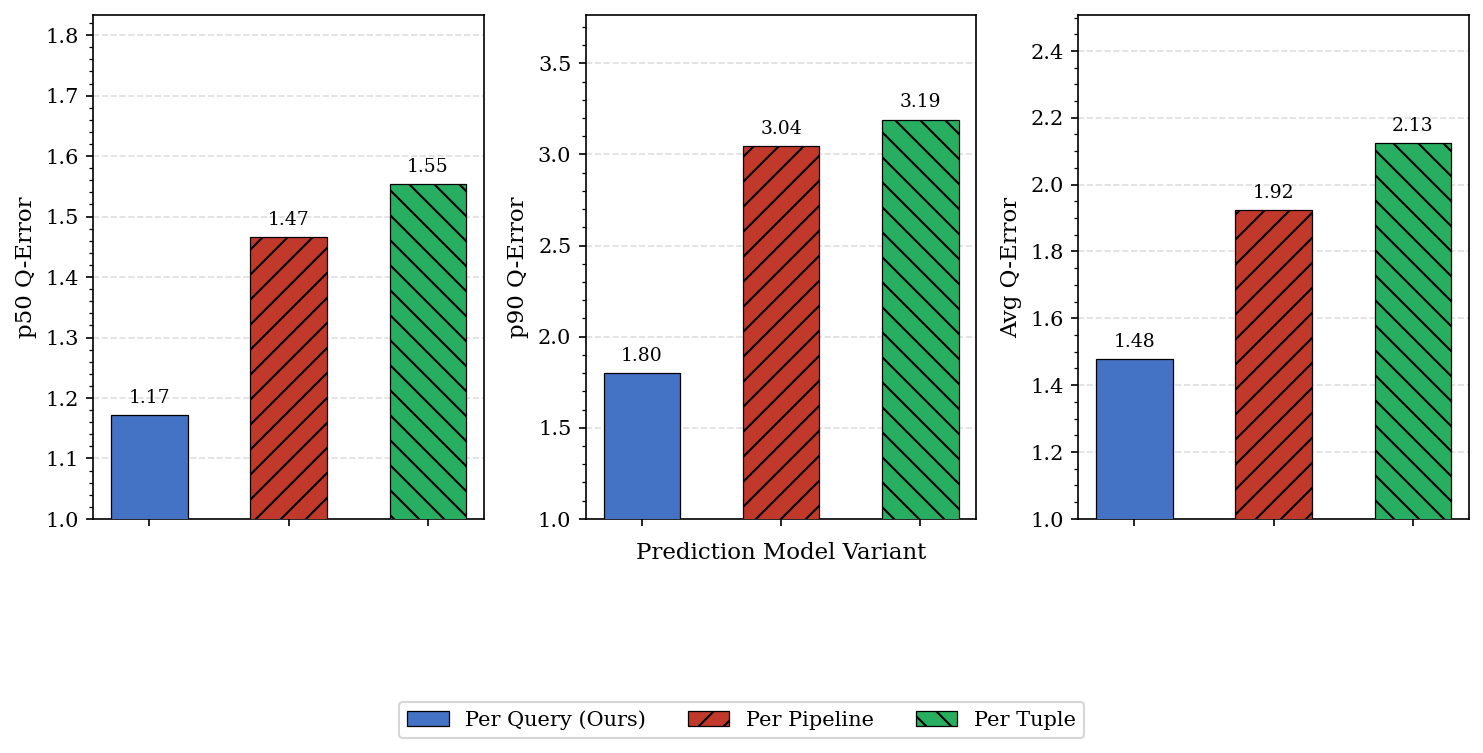
\includegraphics[width=\textwidth]{figures/query_pipeline_tuple.png}
  \caption[Prediction Granularity Comparison]{Q-Error (p50, p90, and average) for three prediction granularities over all queries: per-query, per-pipeline, and per-tuple.}\label{fig:query_pipeline_tuple}
\end{figure}

\begin{figure}[htpb]
  \centering
  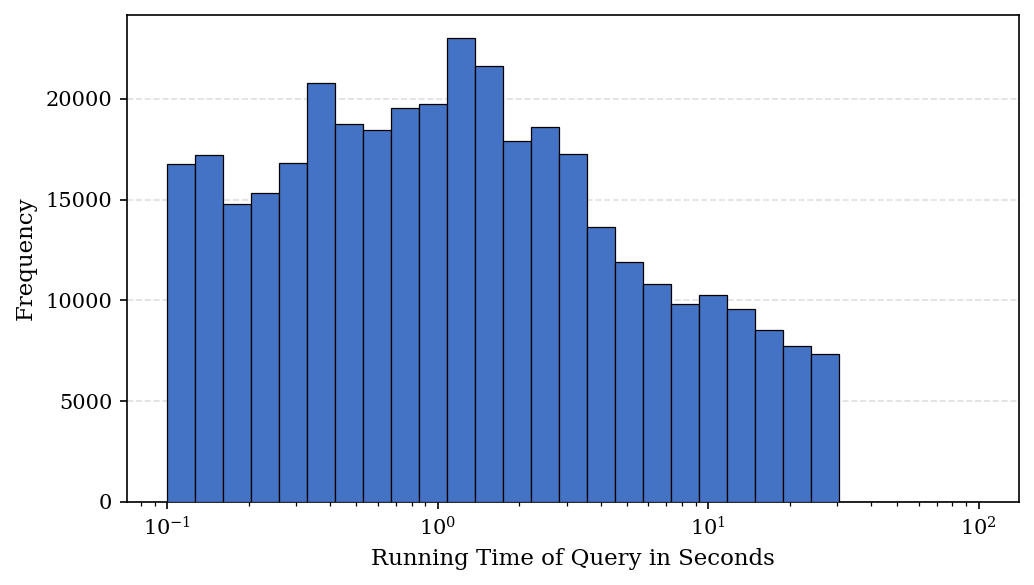
\includegraphics[width=\textwidth]{figures/query_runtime_hist.png}
  \caption[Query Runtime Distribution]{Distribution of all query running times of the ZeroShot dataset.}\label{fig:query_runtime_hist}
\end{figure}

